\chapter{Design \& implementation}
In the previous chapter we described some of the available stream processing frameworks. We evaluated some of them and eventually we decided to integrate Apache Flink in Cowbird. In this chapter we are going to illustrate how SWAN-Songs evaluation can be ported to Apache Flink. More in general, we will portray how we extended Cowbird in order to accommodate sensors data sensing and SWAN expressions evaluation on a large scale. We will discuss the design choices we made and the technical challenges we tackled.  

\section{Distributed Cowbirds}
The existing Cowbird framework is not suitable for processing large number of SWAN-expressions in real-time with possibly high-frequency data sensors.
We designed a distributed architecture for supporting the real-time evaluation of a massive number of SWAN-Song expressions in Cowbird. We extended the Cowbird cloud architecture (see figure \ref{fig:distributed_cowbirds}) adding two main components:
\begin{itemize}
\item \emph{Cowbird Fog}. A distributed layer responsible of receiving SWAN-Song evaluation requests from smartphones, polling sensors data and computing expressions. It is designed to bring expressions evaluation as close as possible to the data generation in order to reduce latency. The Fog layer can decide to offload the SWAN-Song evaluation to the Streams layer according to some expression parameters (e.g. sensors data generation frequency, SWAN expression time window). If an expression is offloaded to the Streams layer, the activated sensors threads in the Fog layer will publish their sensed data to a Kafka broker that mediate communications between the Fog and the Streams layer.
% GEOGRAPHICALLY STUFF
\item \emph{Cowbird Streams}. A high-performance and scalable layer for evaluating SWAN-Song expressions in real-time on a cluster using Apache Flink. It evaluates sensors sensed data provided by the Fog layer and streamed through the Kafka broker. The result of the evaluation is sent back to Kafka and then made available to the Fog.
\end{itemize}

 \begin{figure}[h!]
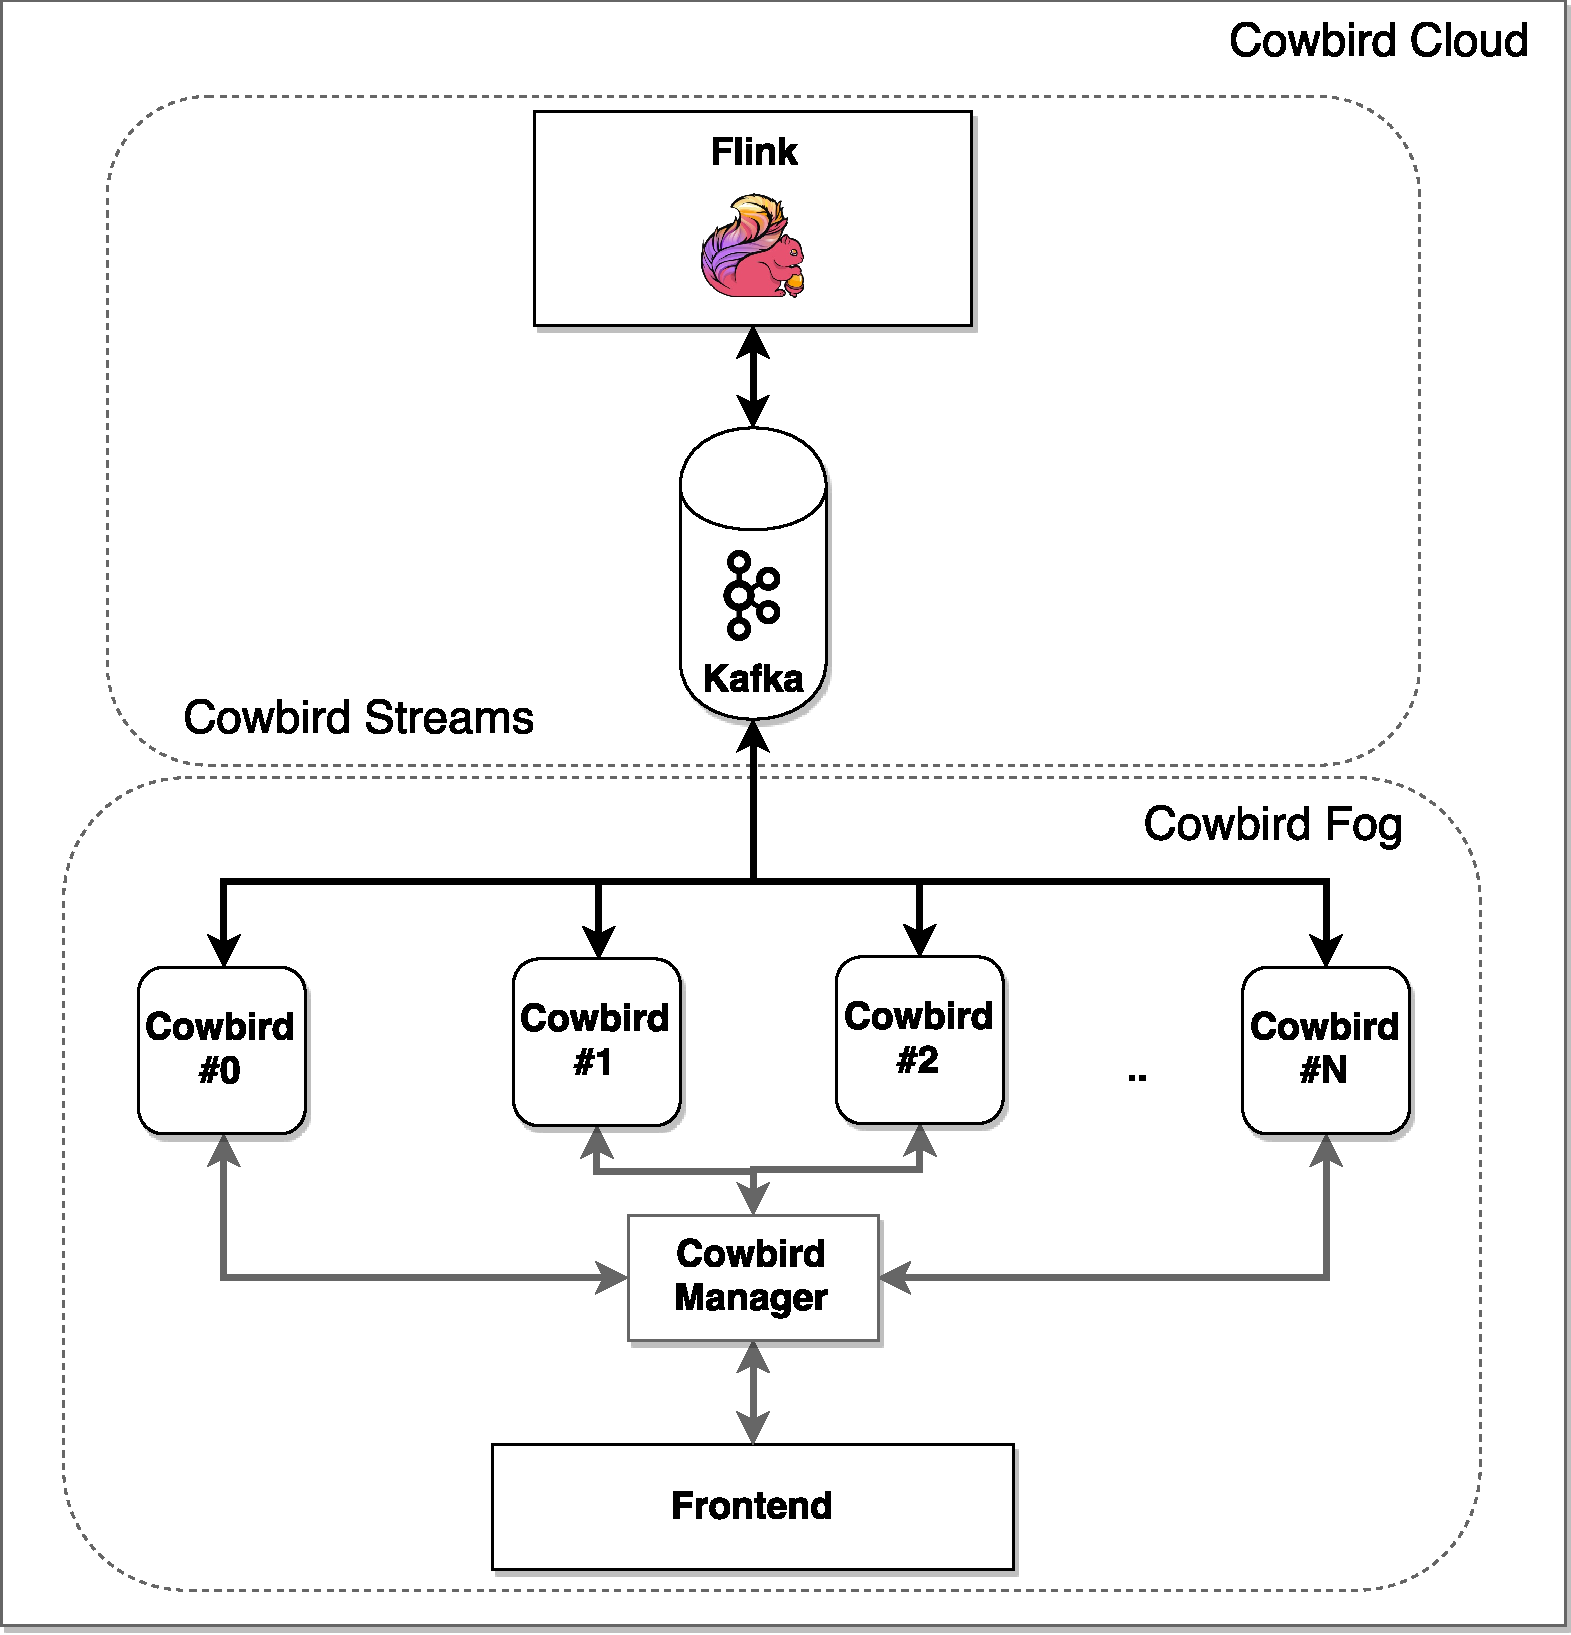
\includegraphics[width=1\textwidth]{images/cowbird_distributed.pdf}
 \caption{Distributed Cowbirds cloud architecture}
\label{fig:distributed_cowbirds}
\end{figure}

The Distributed Cowbirds model differs from the other streaming architectures described in Chapter 2. We called the Distributed Cowbirds a \emph{hybrid} architecture since it combines large-scale modern streaming analysis techniques with more traditional processing mechanisms. In fact, we added the Fog layer for performing some relative simple evaluation without involving an actual cluster system. The Fog layer can reduce latency bringing computation close to the data generation and to the users (and their smartphone). In fact, the Fog layer could be geographically distributed in order to provide high availability and high performance while the Streams layer could be a more centralized entity of the architecture used for more complex evaluations that the Fog cannot handle. Furthermore, the Fog layer is extremely portable since it could be deployed on any device that runs a JVM. 

The remainder of this chapter will describe the internal details of the Distributed Cowbirds architecture. 

\section{Cowbird Fog}
In Chapter 1, we have seen that Cowbird makes large usage of threads for polling sensors data from external endpoints. This approach allows Cowbird to poll many different sources concurrently and in an asynchronous fashion. In Cowbird, a multi-threaded mechanism is adopted also for the SWAN-Song expressions evaluation. However, having many active threads on a single computing node can incur in a certain system overhead. Furthermore, when polling live data, fetching data values might be delayed as new data records are available as Cowbird needs to wait for the relative sensor thread to become active again. A delay in fetching the data will induce a delay in processing the expression. In reaction to these issues, we decided to \emph{scale horizontally} the Cowbird cloud instance. 

The Cowbird cloud instance is built using the Play framework with Java. For these reasons, we decided to scale out Cowbird using Akka \cite{akkaonline}. Akka is a set of open source libraries for building highly concurrent, distributed, and resilient message-driven applications using the \emph{actor model} \cite{actormodelbook}. The \emph{actor} is the primitive building block that forms the basis of the actor model. An actor is a concurrent entity that keeps an internal state that is not shared with other actors. The actor propagate data or events with other concurrent entities explicitly via asynchronous messages without blocking. Each actor processes the receiving messages one by one and it modifies its internal state. An actor is usually mapped to a thread; multiple actors can actually share the same system thread. The Actor model, because of its simplicity by design, can scale from processor cores to networks.

In the original Cowbird implementation all its functionalities such as as receiving SWAN-Songs evaluation requests, sensing sensors data and computing the expressions are abstracted as a single instance. In the new distributed architecture, we structured the Cowbird Fog layer as follows:
\begin{itemize}
\item \emph{Frontend}. The Frontend is in charge of receiving the SWAN-Song expressions evaluation requests from smartphones. The Frontend mainly consists in the Play framework controller of the original Cowbird implementation that routes a specific URL to a functionality. The Frontend is managed by the Frontend Manager. Every time a SWAN-expression evaluation request is received at the Frontend, the Frontend Manager will spawns a \emph{frontend actor} responsible of the communication between the Frontend and the Cowbird manager. In particular, the frontend actor registers the SWAN-Song to the Cowbird manager and it will be notified when a new result value for the expression is available. Scenario with multiple Frontend instances are possible and supported by the system.

\item	 \emph{Cowbird node}. The Cowbird manager assigns SWAN-Songs expressions to be evaluated to a Cowbird node. The Cowbird node when receiving a SWAN expression, through the evaluation engine, will start the relevant sensor thread that will keep polling external web data from an endpoint. When the Cowbird node compute new results for a registered SWAN expression, it will send back the results to the Cowbird manager; the result is sent back to the manager with the same communication optimization strategy described in Chapter 1. The Cowbird node runs a \emph{remote evaluation manager} that determines whether or not a SWAN-Song expression should be offloaded for evaluation to the Cowbird Streams layer. A SWAN-Song expression (or just a part of it) is offloaded to the Streams layer if it refers to a sensors marked as \emph{high-frequency} or if the expression has to be evaluated over a time window that is longer of a certain configurable threshold (e.g. 10 minutes).

The Cowbird node integrates a Kafka \emph{producer} and a Kafka \emph{consumer} that coordinate the communication with the Streams layer. 

Cowbird nodes can be dynamically added or removed for horizontal scalability.

\item \emph{Cowbird manager}. The Cowbird manager is responsible for the coordination of the workload distribution among all the Cowbird nodes in the system. When a new SWAN-Song expression evaluation request is received from the Frontend, the manager assigns it to \emph{least-busy} (i.e. the Cowbird node with the minimum number of active threads) Cowbird node in the network. The Cowbird manager is also responsible of monitoring the entire Fog layer. In fact, the manager detects failing Cowbird nodes and Frontend(s). In reaction to these scenarios, the manager can redistributes the workload to another active node in the system or it can stop the sensors data sensing and expression evaluation in case of a failing Frontend. The Cowbird manager can be deployed in \emph{high-availability mode} to guarantee a certain level of fault-tolerance. In such scenario, when the manager fails one of the Cowbird node will be elected as the manager. 
\end{itemize}

Because of the Akka framework flexibility the above described components can be deployed all three in a single machine or they can be distributed over many computing nodes for achieving better performance. Scenarios where different Fogs are distributed geographically for performance and availability are possible. Hence, Cowbird cloud would meet the concept of \emph{fog computing} \cite{fogcomputingBonomi2012}. 
%GEOGRAPHY

\section{Cowbird Streams}
The Cowbird Streams layer is the high-performance module of the our new Cowbird implementation. As we already mentioned, it consists of a Kafka cluster and an Apache Flink application. The Kafka cluster is responsible of receiving the sensed data from the Fog layer; the Flink application processes the incoming streams and write the result of the evaluations back to Kafka.

We ported the SWAN-Song evaluation mechanism to Apache Flink. In particular, we implemented the core SWAN-Song functionalities using the Flink API. In order to bring SWAN-Song evaluations on top of Flink, we need to stream the registered expressions along with the sensed data from the Fog layer through Kafka. The Fog layer exchanges \emph{messages} with the Flink job running the SWAN logic. All the messages are exchanged in JSON format through the Kafka broker. We designed three different type of messages:
\begin{itemize}
\item \emph{Sensor message}. Every time a sensor thread that belongs to a SWAN-Song assigned for evaluation to the Streams layer generates a data record it is encapsulated in a sensor message. The sensor message contains the data value and the identifier of the expression it belongs to. In fact, each SWAN-Song expression has an unique identifier assigned by the Cowbird manager.
\item \emph{Control message}. The control message is sent from the Cowbird manager when it wants to register/deregister a SWAN-Song expression to the Streams layer. It contains the identifier of the expression and the type of history reduction along with the window size.
\item	 \emph{Result message}. The result message contains the result of the evaluation. It is sent from the Flink job every time a new result is available for a certain expression.  
\end{itemize}

When the Cowbird node receives a new expression to evaluate from the Cowbird manager, the remote evaluation engine evaluates if the expression or part of it should be evaluated by the Streams layer. If this is the case, the Cowbird node will register the SWAN-Song through a control message to the Streams layer. The evaluation engine will then start the relative sensors threads; the sensed data instead of being stored and evaluated locally will be sent to the Flink job running on the Cowbird Streams. The Cowbird node will be notified when a new result for the registered expression is available.
\subsection{SWAN-Song evaluation on Cowbird Streams}
Implementing the entire SWAN logic on top of a streaming engine can be very inefficient. SWAN expressions are parsed by the Cowbird Fog and parsing them again would introduce extra overheads. 
% the expression on the Streams layer  Implementing from scratch the entire SWAN stack functionalities (e.g. parsing expression, expression evaluation) on Apache Flink would require a lot of effort and it would be probably useless. 
Thus, we designed the system in a way the Fog layer can offload only some \emph{well-known} type of SWAN expressions (or subexpressions of a more complex expression) to the Streams. The Fog layer will be then in charge to compute the final result of an expression with the partial results computed by the Streams layer. In particular, our Streams layer is capable of computing the following type of SWAN-(sub)expressions: SWAN simple value expression, SWAN simple tristate comparison expression and SWAN complex tristate comparison expression. 

\subsubsection{SWAN simple value expression} 
This is the simplest kind of SWAN-Song expression that can be evaluated by the Cowbird Streams layer. Such expressions only contains the basic SWAN predicates but they don't support the ALL or ANY reduction mode. An example of such expressions can be:
\begin{equation}\label{eq:simpleexpression}
cloud@thingspeak:field?channelid='1'\#field='1'\big\{MEAN,3600000\big\}
\end{equation}

If a SWAN simple value expression is part of a more complex expression, the final result would be computed by the Fog layer when the result of the simpler expression is evaluated on the Streams and then sent back. For example, consider the following expression:
\begin{equation}\label{eq:simpleexpression_comparison}
cloud@thingspeak:field?channelid='1'\#field='1'\big\{MEAN,3600000\big\} > 50.0
\end{equation}

In SWAN-Song \ref{eq:simpleexpression_comparison} only the left-side of the expression would be offloaded to the Streams layer. The final comparison (if the MEAN value is greater than 50) would be computed on the Fog layer when the result of the left-side expression is received back.

\subsubsection{SWAN simple tristate comparison expression} 
The SWAN simple tristate comparison expression is a comparison expressions that consists of a SWAN-Song expression with ANY or ALL history reduction mode and a constant value. For example, consider the following expression:
\begin{equation}\label{eq:simple_comparison_expression_comparison}
cloud@thingspeak:field?channelid='1'\#field='1'\big\{ANY,3600000\big\} > 50.0
\end{equation}

The expression \ref{eq:simple_comparison_expression_comparison} is completely evaluated on the Streams layer and when a result is available is pushed back to the Cowbird Fog layer. This approach is essential in order to prevent the Cowbird Streams layer to return a long list of time-stamped values. 

In order to maximize efficiency and perfomance some shortcuts have been implemented in the evaluation of such expressions. In particular, in case of a simple comparison expression that has the ANY history reduction mode the expression is evaluated immediately (without waiting for the other sensor values generated within the window history length) when a data record that makes the expression TRUE flows into the Streams layer. On other hand, a simple comparison expression that has the ALL history reduction mode is immediately evaluated if a record that makes the expression FALSE enters the system.


\subsubsection{SWAN complex tristate comparison expression} 
The SWAN complex tristate comparison expression represents a more complex type of comparison expression. It consists in comparison expressions that involve the ANY or ALL history reduction modes. For example, consider the following expressions:
\begin{equation}\label{eq:complex_comparison_expression_comparison}
cloud@mysoundsensor1\big\{ANY, 3600000\big\} > cloud@mysoundsensor2\big\{ALL, 2400000\big\} 
\end{equation}
The expression \ref{eq:complex_comparison_expression_comparison} is completely evaluated on the Cowbird Streams layer (if offloaded).

\subsection{SWAN-Song streaming-oriented evaluation}
The new Cowbird implementation supports the same set of operations provided by the previous generation of Cowbird cloud. In fact, offloading the three types of (sub)expressions described above to the Streams layer and let the Fog layer computing and aggregating the partial results (if applicable) leads to the same exactly result.

The SWAN features are implemented on Apache Flink using its low-level operations API (i.e. ProcessFunction). The Flink implementation keeps an internal state for each stream of sensors data using the RocksDB key-value store \cite{rocksdbonline}. This state backend can store very large state that exceeds memory and it spills to disk efficiently. All the SWAN features are implemented in Apache Flink using \emph{processing time} in order to guarantee real-time performance even if data records are delayed. However, event time can be configured by the user.

We designed two different implementation of how the Cowbird Streams processes SWAN-Song simple value expressions. One implementation, that we called \emph{core implementation}, reproduces exactly the way SWAN-Songs are processed in the original SWAN framework. In particular, for each expression the system collects all the sensors values generated within the history time window and the history reduction mode is then applied. This approach is very precise and it allows the system to continuously generate an expression result based on the values stored that belong to the history time window. However, this approach is not really \emph{streaming-oriented}; in fact, streaming applications should incrementally aggregate partial results while new data records enter the system. This approach can prevent the system to leave the ground to the back pressure effect and it drastically reduces the amount of storage required by each stream for keeping its internal state. In reaction to this, we designed a \emph{streaming-oriented} SWAN-Song evaluation that can be executed on Cowbird Streams. The philosophy of this implementation is to store the partial results of each stream of data related to a SWAN-Song expression instead of all the data values generated by the sensor within a certain history time window. For example, if we want to compute the MEAN value of the data generated by a sound sensor in the last five seconds we just need to count how many data occurrences have been generated by the sensor and the sum of the data values. Another example can be an expression with the MAX history reduction mode set. In this scenario, we just need to store a partial maximum value and every time a greater value enters the system we can simply replace the partial maximum. This approach can drastically reduce the space complexity of our streaming application; complexity that could explode when we deal with very large streams of data. 

The MAX, MIN, MEAN history reduction modes can very easily adopt this streaming-oriented evaluation approach. However, the MEDIAN operator requires all the data records in order to compute the median value. We decided to design a MEDIAN operator implementation that approximates the median of the data streams. In the literature, there are many approaches designed to approximate sensors values \cite{approximateprobabilistic, approximationdatabase}. These techniques are very attractive for some domains where a large number of sensing devices are involved such as enviromental monitoring, agriculture and industrial monitoring applications \cite{approximationtimeseries}. We approximated the MEDIAN history reduction mode using the remedian algorithm \cite{remedian}. This algorithm has been proven to be very efficient \cite{remedianfurtheranalysis} and it only requires $\mathcal{O}(\log{}n)$ space to compute the median value. This technique can be used for both batch and stream processing. 

The remedian algorithm requires \emph{k} arrays of size \emph{b} that are continuously reused. The data enter at the first array that is filled with the first b observations. Then, the median of these b observations is stored in the first element of the second array. The first array is then used again for the second group of b observations, the median of which will be put in the second position of array 2. After some time array 2 is full too, and its median is stored in the first position of array 3, and so on. When the \emph{k}-th array is complete its median becomes the final estimate. If the input data cannot fill the entire matrix, the estimation of the median is calculated as a \emph{weighted median} of the stored data. In particular, the $n_1$ numbers in the first array have weight 1, the $n_2$ numbers in the second array have weight b, and the \emph{$n_k$} numbers in the last array have weight $b^{k-1}$.

In our SWAN-Song streaming oriented evaluation implementation, the k and b value of the remedian matrix can be configured by the user. However, we set as default values k=15 and b=11 as described in \cite{remedian}. With these values our system is able to process the (re)median value of a stream of data that has up to $11^{15}$ observations with just a $11 \times 15$ matrix. 

The SWAN-Song streaming-oriented evaluation is much more efficient than the traditional implementation and it is more suitable for real-time streaming applications. However, the new implementation introduces a lower degree of accuracy for the MEDIAN operator. Furthermore, the SWAN-Song streaming evaluation operates only over \emph{fixed} or \emph{aligned} time windows (i.e. the reduction is applied only across all the data ingested during the window of time in question). In fact, since the reduction is calculated continuously aggregating incoming data within a time frame, an expression result is emitted at the end of each time window. 

The SWAN-Song streaming-oriented evaluation is particularly suitable for applications that can tolerate a certain lack of accuracy and that operate at regular time intervals. Mission critical applications, where a better level of accuracy is required, could instead use the traditional implementation. Both the implementations are available in the Cowbirds Streams layer and they could be deployed together allowing different type of sensors to use the most convenient evaluation strategy.

\section{Recap}
In this chapter we described how we extended the existing Cowbird cloud instance for supporting a massive volume of SWAN-Song expression evaluations. We called the new Cowbird architecture \emph{hybrid} since it adds an extra computational layer to the traditional streaming architecture.

The Cowbird Fog module brings the evaluations closer as possible to the sensors data generation. The Fog layer is also extremely scalable since Cowbird nodes can be dynamically added and removed at run time. Furthermore, different Fogs could be geographically distributed for high-availability and better performance. 

The Cowbird Streams is the high-performance and large-scale component of the architecture. The Streams layer is powered by Apache Flink that we demonstrated to be the streaming framework that best meets our scenario. The Cowbird Streams supports two different SWAN-Song evaluation strategies: a core implementation that exactly reproduces the SWAN framework and a more \emph{streaming-oriented} implementation. Both implementations can be adopted according to the type of sensor  which the data is being evaluated. The Cowbird Streams is designed to accommodate \emph{long-running} SWAN-Song expressions or expressions characterized by very \emph{high-frequency} sensors. 

The Distribute Cowbirds implementation is available at \url{http://github.com/gdibernardo/cowbird-distributed}.


